% Created 2017-02-08 mié 12:22
% Intended LaTeX compiler: pdflatex
\documentclass[11pt]{/home/hao/dev/org/latex-plantilla/IEEEtran}
\usepackage[spanish, mexico]{babel}
\usepackage{url}
\usepackage{minted}
\addto\captionsspanish{\renewcommand{\contentsname}{Contenido}}
\usepackage[utf8]{inputenc}
\usepackage[T1]{fontenc}
\usepackage{graphicx}
\usepackage{grffile}
\usepackage{longtable}
\usepackage{wrapfig}
\usepackage{rotating}
\usepackage[normalem]{ulem}
\usepackage{amsmath}
\usepackage{textcomp}
\usepackage{amssymb}
\usepackage{capt-of}
\usepackage{hyperref}
\author{Eduardo Vázquez Díaz \\ lalohao@gmail.com}
\date{\today}
\title{Verificación de circuitos digitales con software libre}
\hypersetup{
 pdfauthor={Eduardo Vázquez Díaz \\ lalohao@gmail.com},
 pdftitle={Verificación de circuitos digitales con software libre},
 pdfkeywords={},
 pdfsubject={},
 pdfcreator={Emacs 25.1.1 (Org mode 9.0.3)},
 pdflang={Spanish}}
\begin{document}

\maketitle
\tableofcontents

\begin{abstract}
Se creó una maquina virtual con \emph{Ubuntu Desktop 16.04.1} \uline{LTS} en un
contenedor utilizando el software de virtualizacion \texttt{Qemu}, donde
posteriormente se instaló \texttt{verilator} y \texttt{gtkwave}; a partir de este
sistema se exponen algunas técnicas para simular circuitos con
verilog/C++, además de visualizar las ondas generadas de manera
gráfica.
\end{abstract}

\section{Introducción}
\label{sec:org1bd0044}
La importancia de probar los circuitos antes de ser llevados al
silicio puede representar millones de dolares, sin contar el tiempo
invertido en el diseño, y el que se necesitará volver a invertir
para arreglarlo.

En 1990 el lenguaje de descripción de hardware mas usado era VHDL, a
pesar de que solo tenia constructores básicos para probar
(TestBench) los circuitos . Los diseños empezaban a crecer y nuevo
software comercial se creaba para compensar la falta de funciones.
Algunas empresas invertían horas de trabajo para crear su propio
sistema y no pagar los miles de dolares en licencias, una de ellas
llevó a la creación de Accelera que fue la base de SystemVerilog
\cite{spear08_system}.

De la misma manera surgió \texttt{Verilator}, un simulador potente de
Verilog HDL que además es software libre, este compila el código y
lo optimiza para ser simulado rápidamente \cite{verilator-intro}, en
algunos casos es incluso mas veloz que los simuladores comerciales
\cite{verilator-vs-comercial}.

\subsection{Virtualización}
\label{sec:orgf51d1a7}
La maquina virtual permite encapsular el sistema de verificación de
circuitos en un contenedor que no será afectado (y que no afectará)
la maquina utilizada, esto elimina errores que podrian ser causados
al tener instalado software que utilice configuraciones con
variables globales (PATHS) como ocurre con \texttt{HSPICE} y \texttt{Questa SIM}
por ejemplo.

\begin{center}
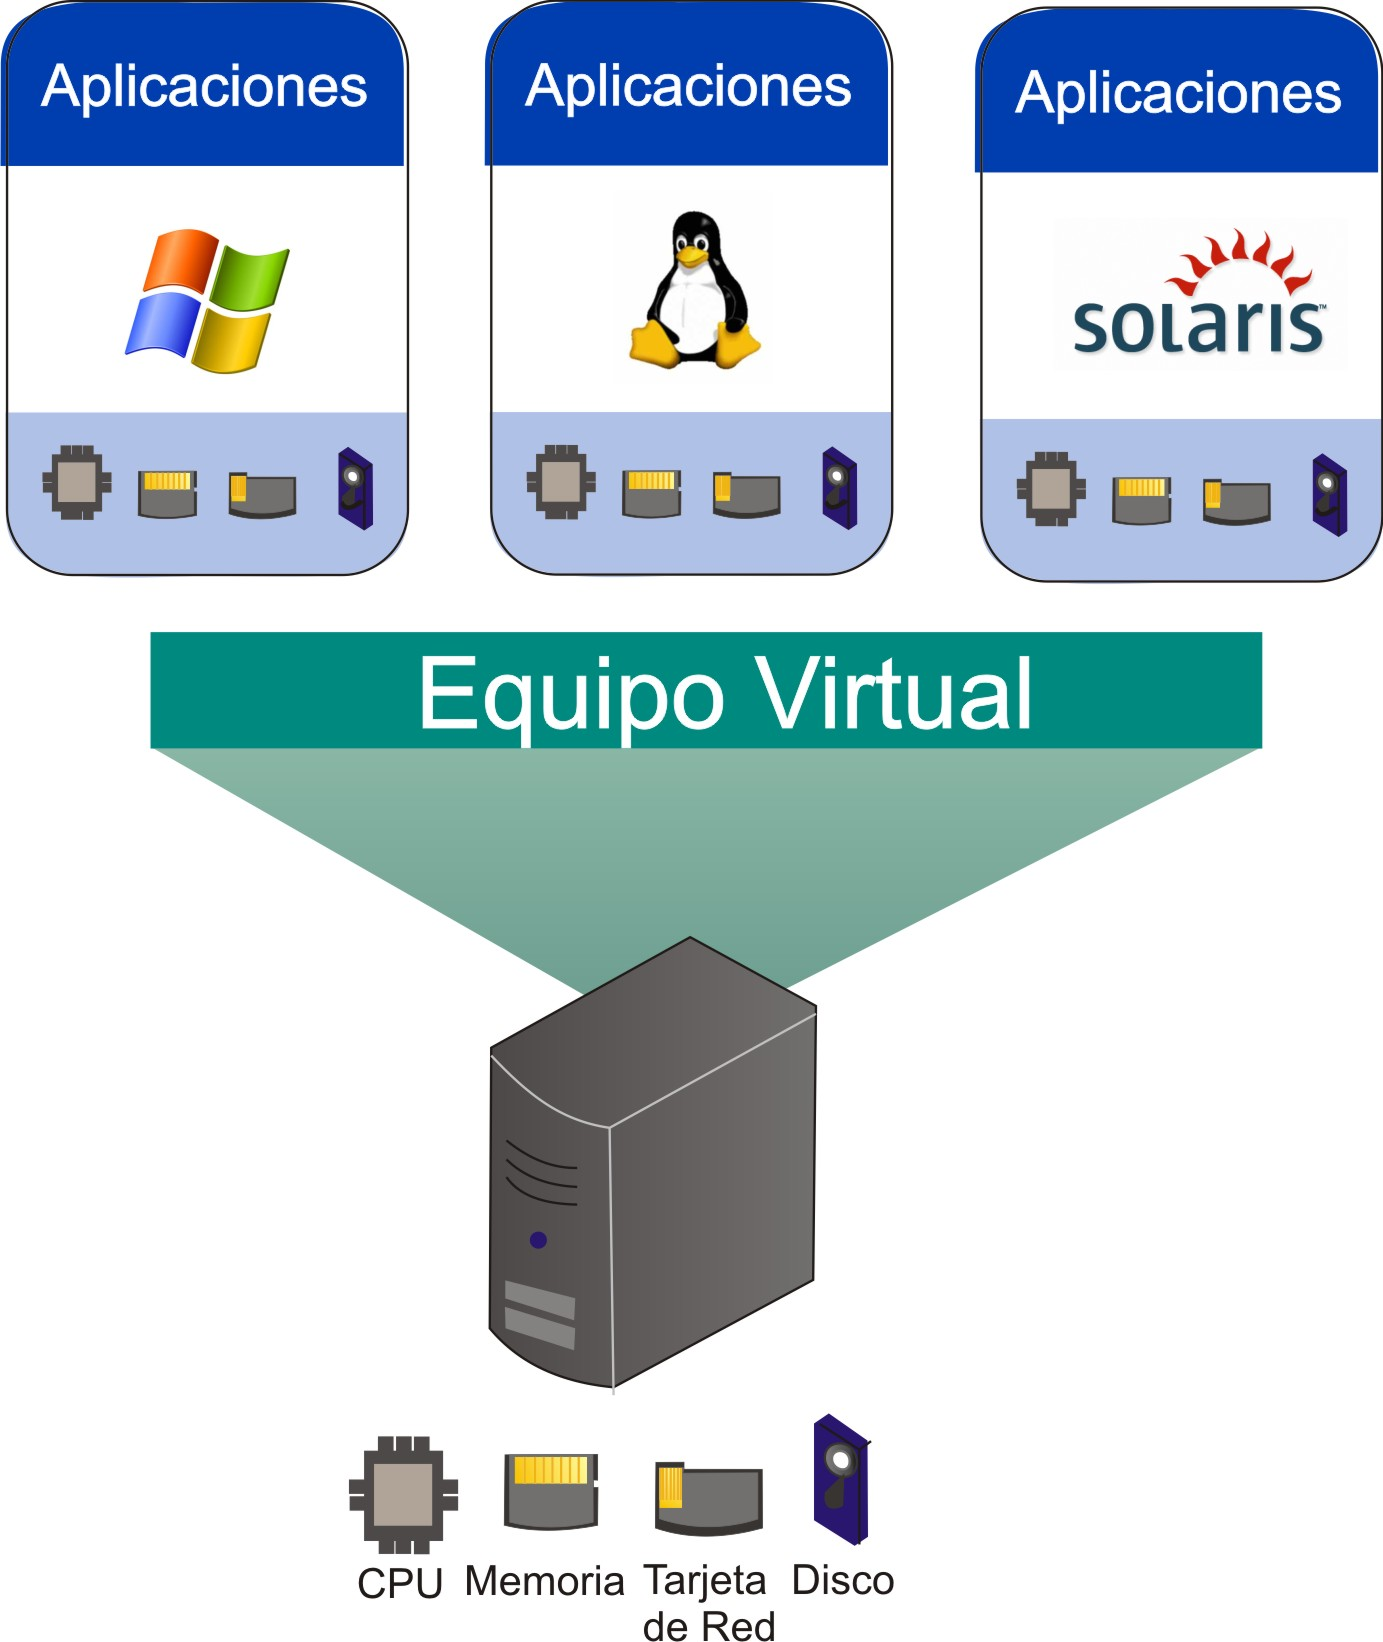
\includegraphics[width=7cm]{virtualizacion.jpg}
\captionof{figure}{\label{fig:org383d342}
Las maquinas virtuales pueden o no conectarse entre ellas o hacia la red externa y pueden ser de diferentes arquitecturas y sistemas operativos independientemente del sistema anfitrion.}
\end{center}

Se le dice anfitrión a la maquina donde se encuentran los
contenedores virtuales, en este caso la anfitriona usa \emph{Arch
Linux}, pero esto no afecta a los contenedores ya que estan
aislados, por lo que esto se puede aplicar de igual manera en
Windows o Mac.
\section{Desarrollo}
\label{sec:orge6e9afe}
Para instalar la maquina virtual se utiliza la linea de comandos,
creando el disco duro virtual llamado \textbf{verif}, con un tamaño de
10Gb, posteriormente se carga el archivo \texttt{ISO} de Ubuntu en el disco
duro creado, con 2G de memoria RAM y se procede a instalar el
sistema operativo de forma normal.

\begin{minted}[]{bash}
qemu-img create -f raw verif 10G
qemu-system-x86_64 -cdrom ubuntu.iso \
                   --boot order=d -drive \
                   file=verif,format=raw \
                   -m 2G
\end{minted}

\newpage
Una vez instalado el sistema operativo se puede iniciar de la
siguiente forma:

\begin{minted}[]{bash}
qemu-system-x86_64 --boot order=d \
   -drive file=verif,format=raw -m 2G
\end{minted}

Posteriormente en la maquina virtual (Ubuntu) se instala el software
necesario para simular \cite{verilator-instalacion}, al igual que el
editor de texto de su preferencia para modificar los archivos :

\begin{minted}[]{bash}
sudo apt-get install git make autoconf \
     g++ flex bison verilator gtkwave
\end{minted}


\bibliographystyle{plain}
\bibliography{bibliografia.bib}
\end{document}